\documentclass[UTF8]{article}
\usepackage{ctex}
\usepackage{listings}
\usepackage[bf,small,indentafter,pagestyles]{titlesec} 

\usepackage{geometry}  %边距和纸张大小
\geometry{a4paper}
\geometry{left=2cm,right=2cm,top=3cm,bottom=3cm}
\usepackage{fancyhdr}
\usepackage{url}
 %使用graphicx包
\usepackage{graphicx}
\usepackage{amsmath}
\usepackage{amssymb} %使用数学符号使用 
\usepackage{cite} %使用引用 
\usepackage{enumerate} %使用item使用

\begin{document} 
\author{    彭峰     05121214   }
 \date{2015-5-10}
\title{忆阻}  %题目要改掉   后面
 \titlespacing{\chapter}{0pt}{*0}{*4}
\titlelabel{\S\thetitle\quad}
\maketitle%这是无目录只有title的部分

\section{前言}
先说说选题原因:还记得当年忆阻在实验室真正被实现时,我通过刊物了解到忆阻这一划时代的器件终于从理论转到实验阶段。还记得当时HP公司说希望在2012年实现成品进入市场。当时还很欣喜,说到时候就能用上这么高端的产品了,未想到现在还是处于实验室阶段,还在研究特性中。。

本次的选题实际上还是有较大的偏移的,忆阻作为第四种元件,虽然也可以当作有“记忆性能的电阻器”使用,但也应该和电阻和电容处于同一层次才是。想想这样和大家的选题不同,大家蜂拥至超级电容器也不是事,加之之前与忆阻的新闻有过一次邂逅,以前也有过了解,还是决定以“忆阻”为选题方向吧。

\section{背景介绍}
从中学和大学基础物理的书籍我们学习了三种主要元器件,分别是电阻,电容和电感,当然学习的时候多以线性元件为基础分析。1971年之前,华裔科学家蔡少棠发现在电流(i)、电压(v),电荷(q)及磁通量($\phi_{B}$)4种变量之间的6种关系有5种是已知的(图\eqref{fig:4})。
\begin{figure}[htbp]
%\centering
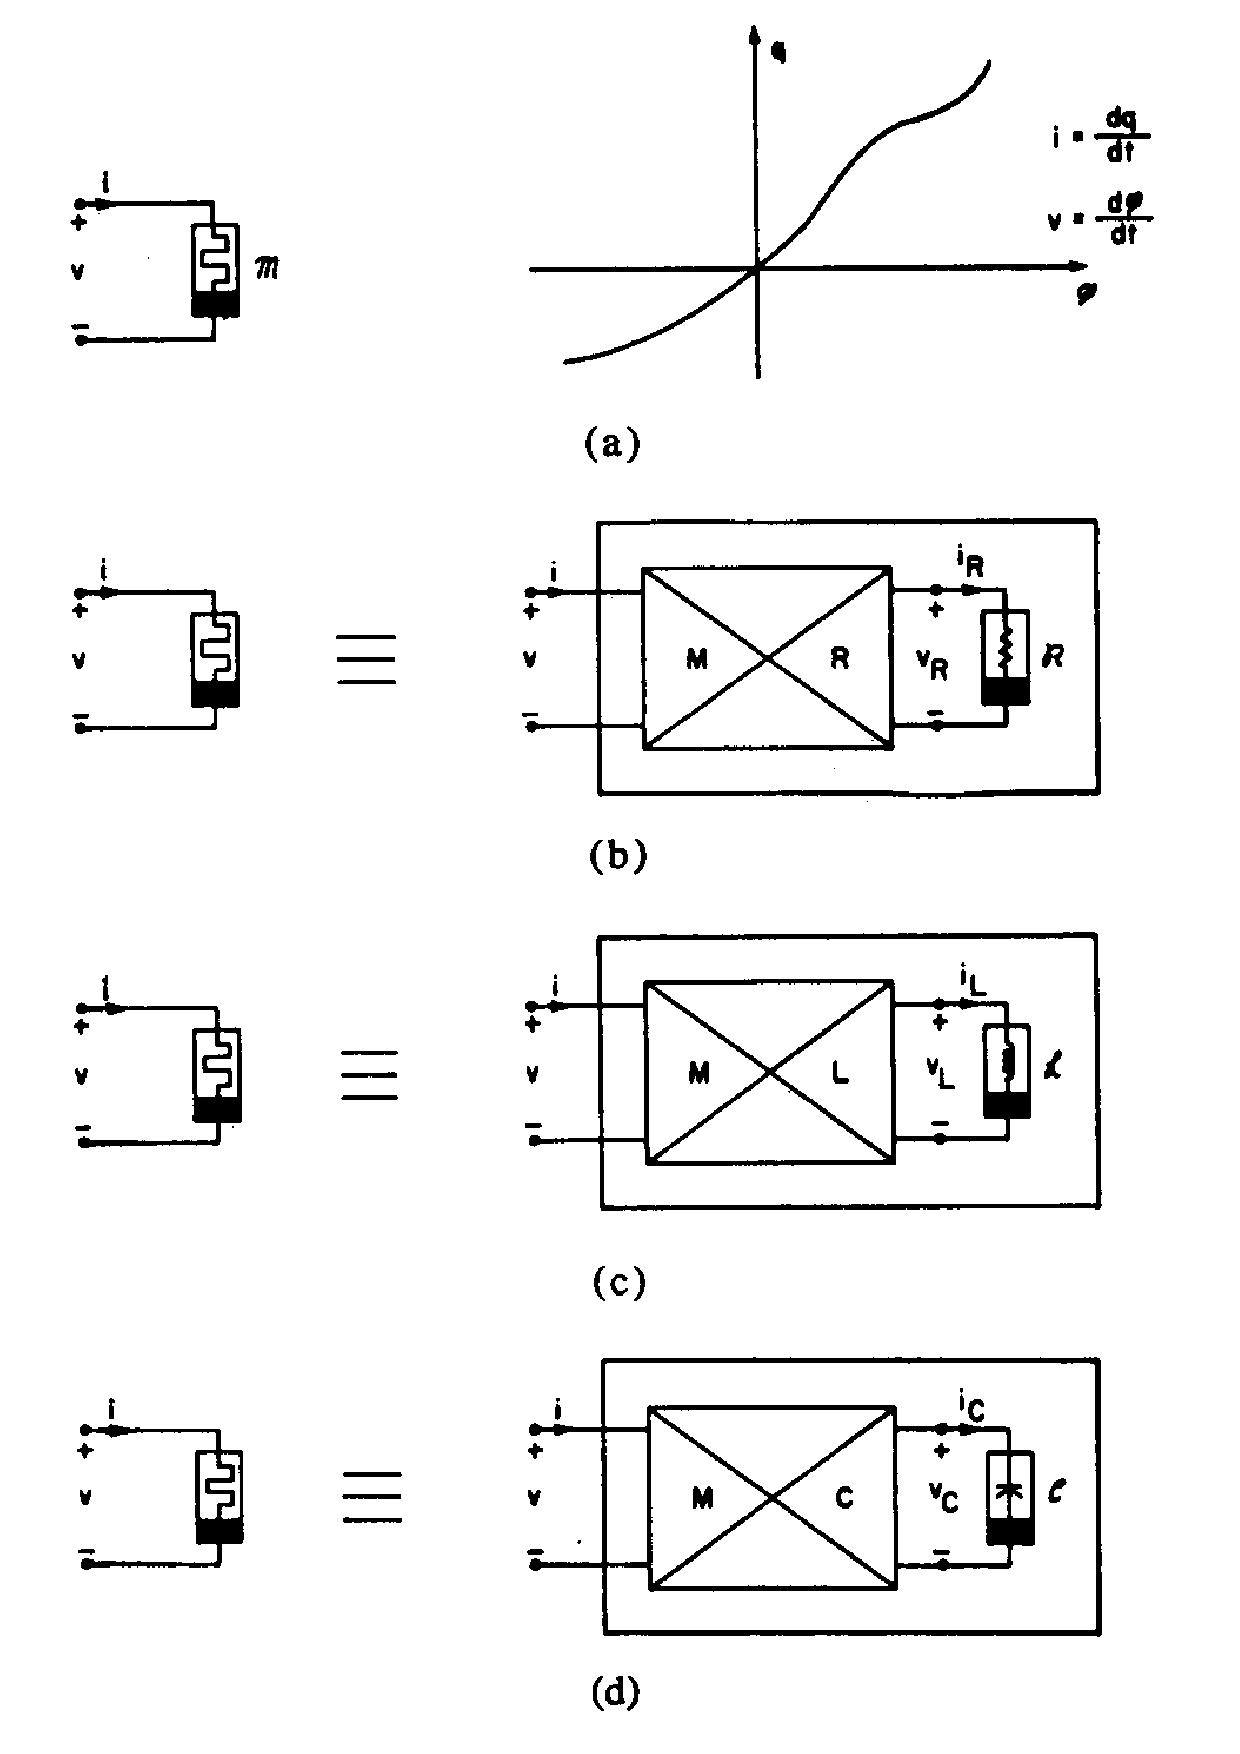
\includegraphics[width=1.77in,height=1.75in]{pic/4}
\caption{三大基本元件物理量关系}
\label{fig:4}
\end{figure}

\subsection{忆阻理论的猜想和提出}
我们知道基于数学的自然理论是和谐的,所以他做了一系列的推断,通过外推对称的非线性电阻(电压与电流),非线性电容器(电压与电荷),和非线性电感(磁通量与电流)之间的的概念,猜想在电阻、电容和电感器之外,应该还有一种组件,代表着电荷与磁通量之间的关系。图\eqref{fig:m1}可以很好地展现四种基本元件的特征。
\begin{figure}[htbp]
%\centering
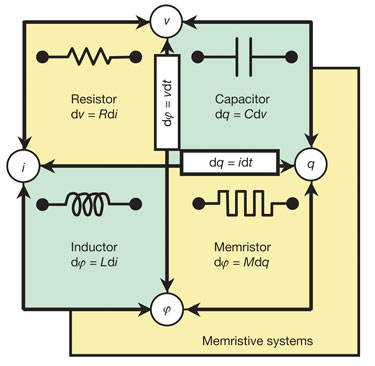
\includegraphics[width=1.77in,height=1.75in]{pic/memristor01.jpeg}
\caption{三大基本元件物理量关系}
\label{fig:m1}
\end{figure}
忆阻理论的提出很好的填补了四种基本物理量关系的空白。然而,这只是基于数学和谐性的猜想,虽然在当时蔡少棠通过普通的电子器件模拟了忆阻并且提出了相关性质,但是忆阻并没有真实在实验室实现。因此当时有人并不相信这种理论,认为这只是电阻和电感的一种结合方式,并不是存在。
事情的转机发生在2008年,HP在实验室偶然合成了这一器件。下面部分图片来自《How We Find Memsistor》一文。

\section{忆阻的发现}
%%下面多添加几个ref,,用moore定律的
从介绍上看,其忆阻的发现存在偶然性。上世纪90年代末,当时惠普公司高级研究员Stan Williams建立了该公司的信息和量子系统实验室,以便开拓未来20年的计算技术。40年来,工业界不断制造基于摩尔定律的更小、更便宜的晶体管。于是,Williams研究团队开始研发越来越小的晶体管,这致使他们考虑当设备缩小到单个分子大小时会发生什么,以及单个原子运动将如何影响其性能。
%%%这个部分要看论文写!!
\subsection{}
\subsection{}

\section{忆阻的性质的探讨}
\subsection{}

\subsection{忆阻的疑惑}
%%%提出记忆电阻,记忆电容和记忆电感三种理论


\section{目前忆阻应用的地方(改题目)}
%%%记得那个部分的提出就放这个地方
\section{忆阻的未来}







\end{document}

